\section{Free Vibrations}
\noindent
Free damped vibrations, like in a massed spring system, are a common application of second order linear ODEs. In a massed spring system, there are three main forces acting on the mass that make up external forces.
\begin{enumerate}[label=\arabic*)]
	\item Acceleration of The Mass -- Since acceleration is the 2nd derivative of position $y(t)$, and Newton's Second Law tells us that $F = ma$, the force from the acceleration of the mass is $my^{\prime\prime}$.
	\item Dampening -- We'll assume that this term is proportional to the velocity, $y^\prime$, and a term $b$. So, the force from dampening is $by^\prime$.
	\item Spring Stretch -- Hooke's Law tells us that the force from a spring is $ky$, where $k$ is some term that gives the spring's "stiffness"
\end{enumerate}
Since we assume that the net force is 0 (that's what free means), our equations is
\begin{equation*}
	my^{\prime\prime} + by^\prime + ky = 0
\end{equation*}

\noindent
Extracting the coefficients and solving the auxiliary equation,
\begin{equation*}
	mr^2 + br + k = 0 \implies r = \frac{-b \pm \sqrt{b^2 - 4mk}}{2m}
\end{equation*}
We will consider two cases. One in which there is no damping ($b = 0$), and one in which there is damping ($b > 0$).

\subsection{Free Undamped Vibrations ($b = 0$)}
\noindent
In this case, our equation simplifies to
\begin{equation*}
	my'' + ky = 0
\end{equation*}
The two roots of ou auxiliary equation are
\begin{equation*}
	r = \pm i \sqrt{\frac{k}{m}} = \pm i\omega
\end{equation*}
So, our solution becomes
\begin{equation*}
	y = C_1\cos{(\omega t)} + C_2\sin{(\omega t)}
\end{equation*}
This is the same $\omega$ from physics that means angular frequency, so the same physics formulas apply, like $T = \frac{2\pi}{\omega}$.\\

\noindent
We can simplify this a bit further. If we think of the $\cos$ and $\sin$ components as being sides of a right triangle like so,
\begin{center}
	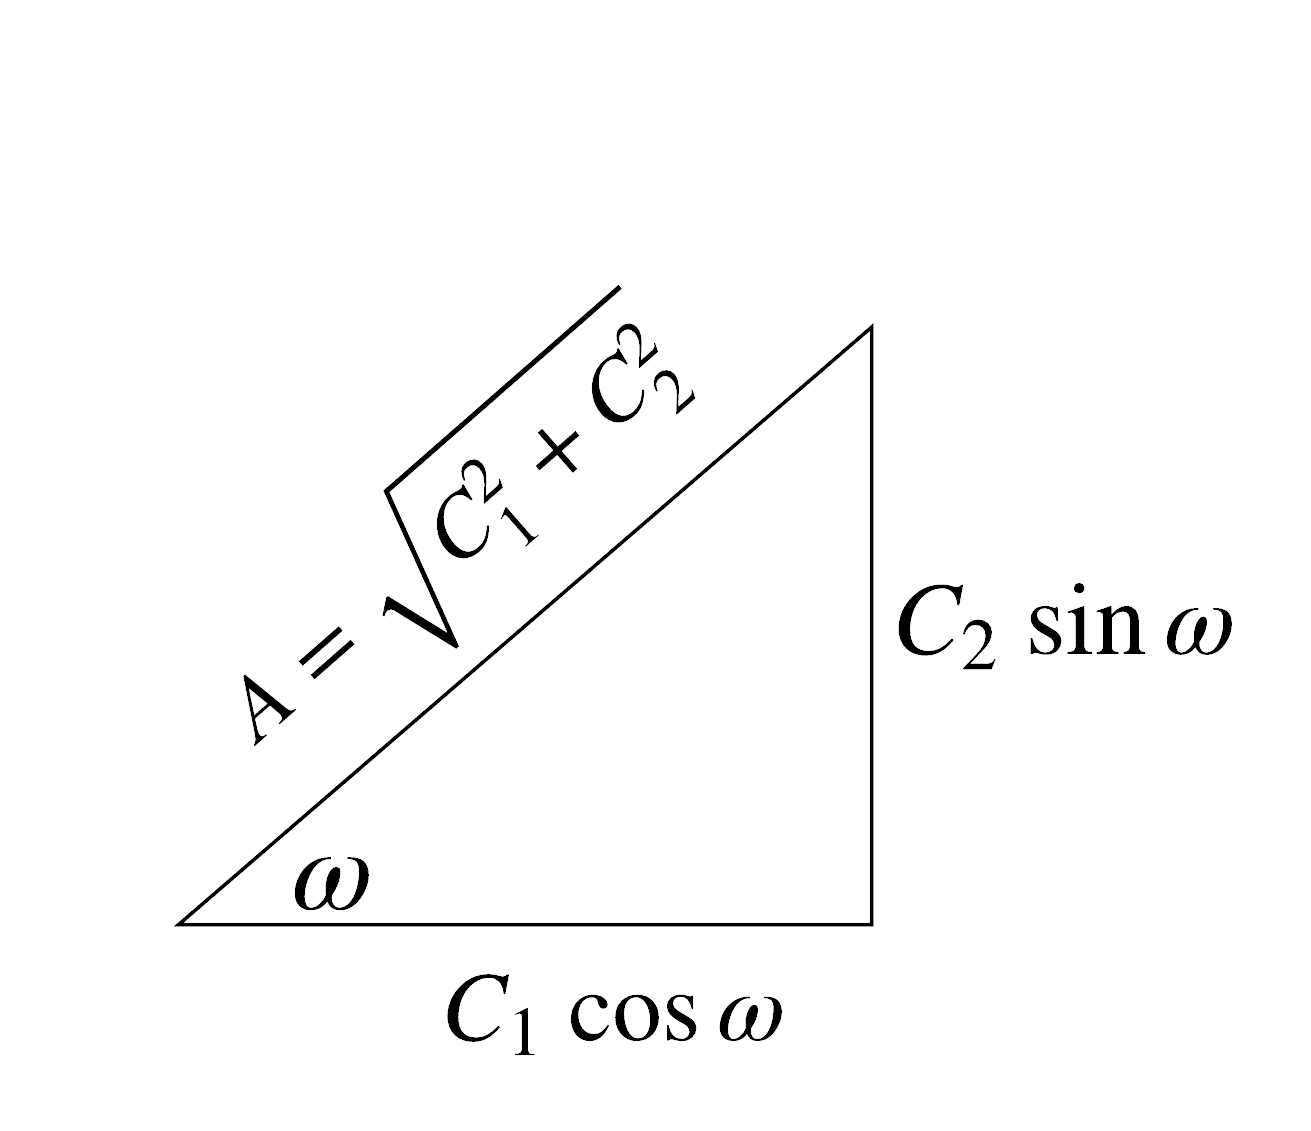
\includegraphics[width=0.5\textwidth]{./higherOrder/freeVibrs/triangle.png}
\end{center}
then we rewrite our equation as
\begin{equation*}
	y = A\left( \frac{C_1}{\sqrt{C_1^2 + C_2^2}}\cos{(\omega t)} + \frac{C_2}{\sqrt{C_1^2 + C_2^2}}\sin{(\omega t)} \right)
\end{equation*}
Note that since $\left(\frac{C_1}{A}\right)^2 + \left(\frac{C_2}{A}\right)^2 = 1$, we can rewrite these coefficients as $\cos{\phi}$ and $\sin{\phi}$ respectively where
\begin{equation*}
	\phi = \begin{cases}
		\arctan{(\frac{C_2}{C_1})} & C_1 > 0 \\
		\arctan{(\frac{C_2}{C_1})} + \pi & C_1 \leq 0
	\end{cases}
\end{equation*} 
So, our equation becomes
\begin{equation*}
	y = A\left(\cos{(\omega t)}\cos{\phi} + \sin{(\omega t)}\sin{\phi}\right)
\end{equation*}
Using the $\cos$ angle addition formula
\begin{equation*}
	y = A\cos{(\omega t - \phi)}
\end{equation*}
\begin{center}
	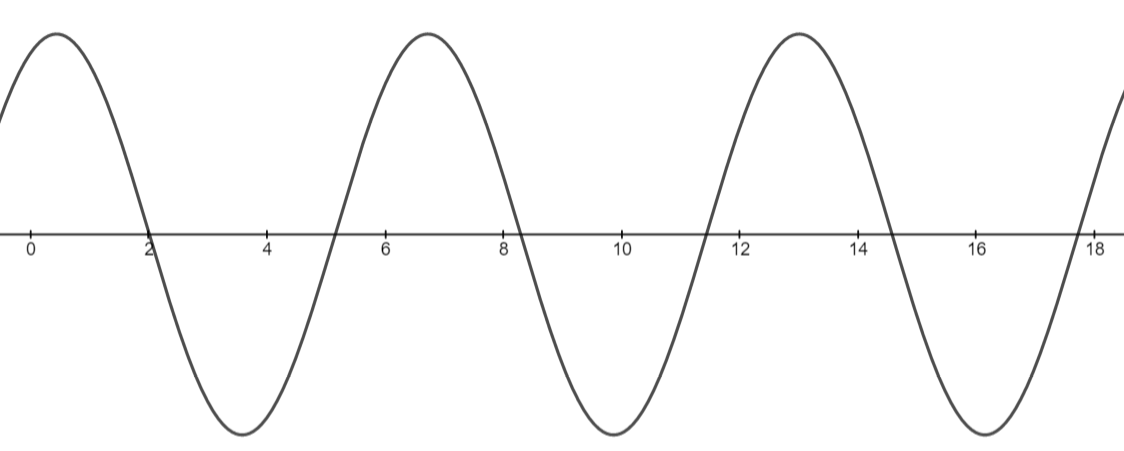
\includegraphics[width=0.5\textwidth]{./higherOrder/freeVibrs/undampedfree.png}
\end{center}
As we can see, an undamped free vibration will simply oscillate back and forth without decay.

\ifodd\includeHigherOrderExamples\begin{example}
	A 2kg mass in an undamped system is attached to a spring with $k = 50 \text{N/m}$. The initial position of the masss is $y_0 = -0.25\text{m}$. The initial velocity is $v_0 = -1\text{m/s}$. Find an expression for $y(t)$, the position of the mass at time $t$. Write your answer in terms of a $\cos$ and a phase shift. Find the period and frequency in proper units.
\end{example}
The IVP describing this problem is
\begin{equation*}
	\begin{cases}
		2y'' + 50y = 0 \\
		y'(0) = -1 \\
		y(0) = -0.25
	\end{cases}
\end{equation*}
Extracting the auxiliary equation and finding the roots,
\begin{equation*}
	2r^2 + 50 = 0 \implies r = \pm 5i
\end{equation*}
So, our general solution is
\begin{equation*}
	y = C_1\cos{(5t)} + C_2\sin{(5t)}
\end{equation*}
Solving for $C_1$ and $C_2$,
\begin{equation*}
	y(0) = -0.25 = C_1 \implies C_1 = -0.25
\end{equation*}
\begin{equation*}
	y' = -5C_1\sin{(5t)} + 5C_2\cos{(5t)}
\end{equation*}
\begin{equation*}
	y'(0) = -1 = 5C_2 \implies C_2 = -0.2
\end{equation*}
Solving for $\phi$, keeping in mind that $C_1 < 0$
\begin{equation*}
	\phi = \arctan{\frac{C_2}{C_1}} + \pi = \arctan{\frac{4}{5}} + \pi
\end{equation*}
So, our answer is (in units of meters)
\begin{equation*}
	y = \sqrt{(-0.25)^2 + (-0.2)^2}\cos{\left(5t - \arctan{\left(\frac{4}{5}\right)} - \pi\right)} \approx 0.32\cos{\left(5t - 3.82\right)}
\end{equation*}
Solving for the period,
\begin{equation*}
	T = \frac{2\pi}{\omega} = \frac{2\pi}{5} \text{s}
\end{equation*}
Solving for the frequency,
\begin{equation*}
	f = \frac{1}{T} = \frac{5}{2\pi} \text{Hz}
\end{equation*}\fi
\subsection{Free Damped Vibrations ($b > 0$)}
We need to consider three cases where the discriminant $\Delta = b^2 - 4mk$ is positive, zero, and negative. 

\subsubsection{Overdamped ($\Delta > 0$)}
This is the simplest and easiest case to deal with because our two roots, $r_1$ and $r_2$, are real and distinct. So, out solution is
\begin{equation*}
	y = C_1e^{r_1 t} + C_2e^{r_2 t}.
\end{equation*}
\begin{center}
	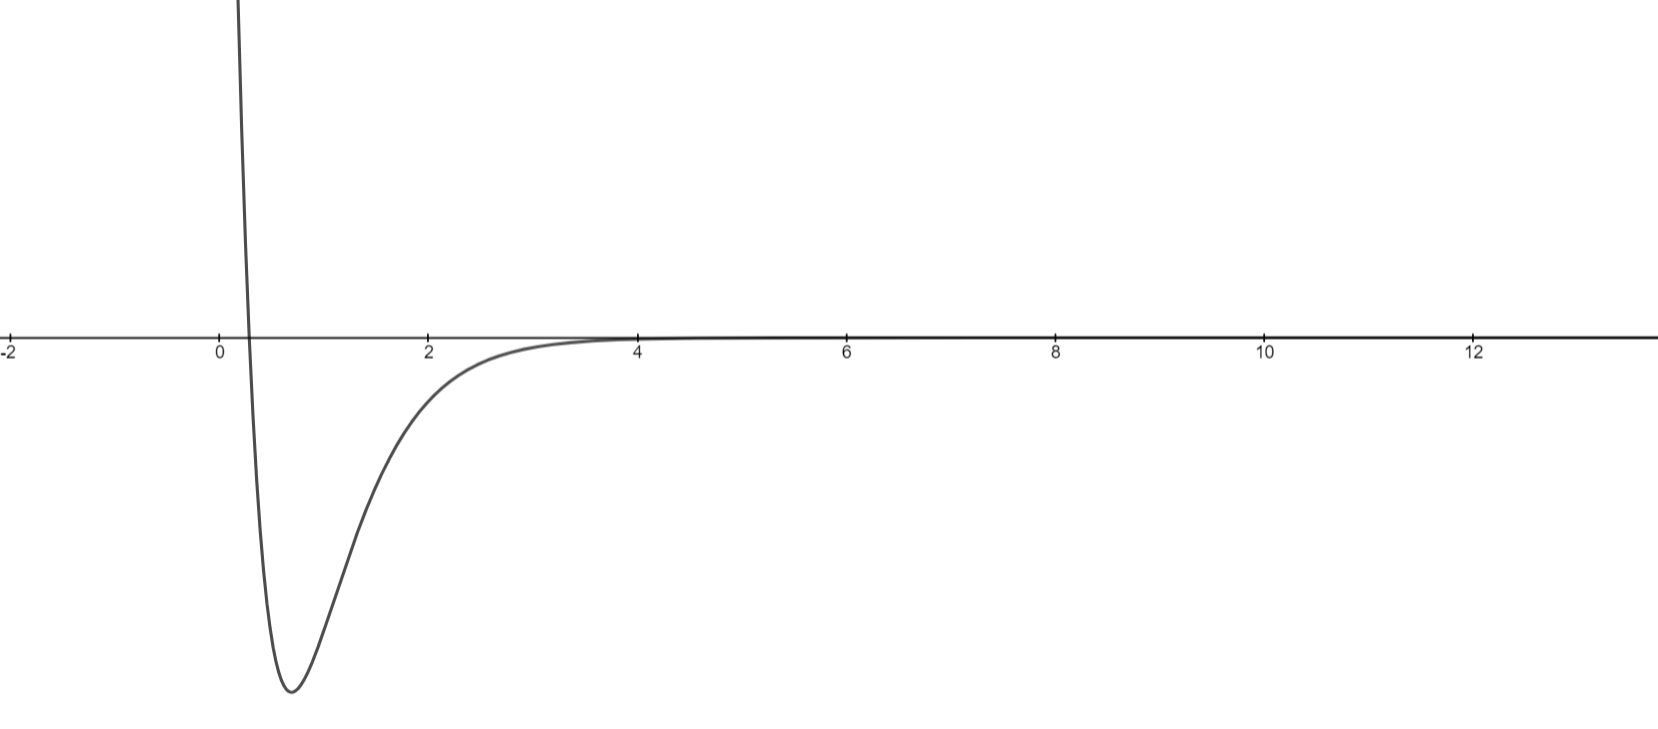
\includegraphics[width=0.5\textwidth]{./higherOrder/freeVibrs/overdamped.png}
\end{center}
We know that $r_1, r_2 < 0$, so
\begin{equation*}
	\lim\limits_{t \to 0}{C_1e^{r_1 t} + C_2e^{r_2 t}} = 0
\end{equation*}
meaning the mass's oscillation decays over time.
\subsubsection{Critically Damped ($\Delta = 0$)}
This case isn't much more difficult. The only difference is that because both roots $r_1$ and $r_2$ are $\frac{-b}{2m}$, we need an extra $t$ term in the solution. So, out solution is
\begin{equation*}
	y = C_1e^{r_1 t} + C_2te^{r_2 t}
\end{equation*}
\begin{center}
	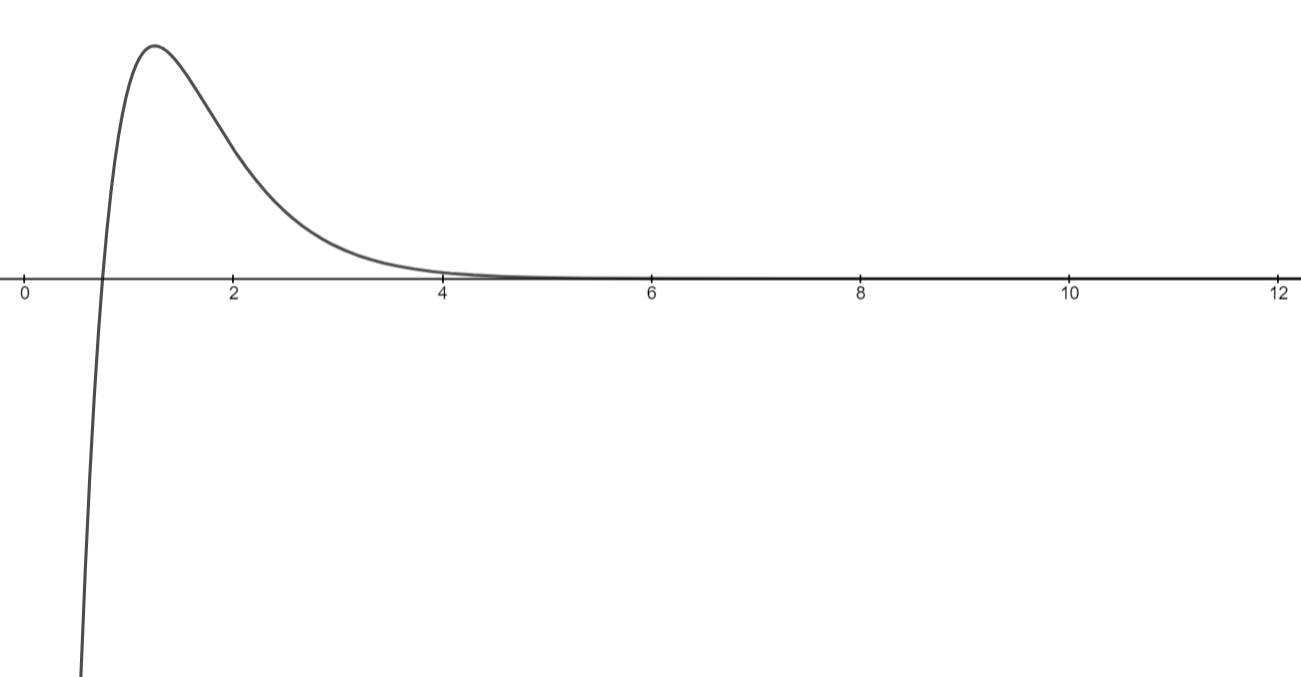
\includegraphics[width=0.5\textwidth]{./higherOrder/freeVibrs/criticallydamped.png}
\end{center}
Since both roots are once again negative,
\begin{equation*}
\lim\limits_{t \to 0}{C_1e^{r_1 t} + C_2te^{r_2 t}} = 0
\end{equation*}
meaning the mass's oscillation decays over time.
\subsubsection{Underdamped ($\Delta < 0$)}
This is probably the most complicated case.
Here, both roots are complex.
Specifically,
\begin{equation*}
	r = \frac{-b}{2m} \pm i\frac{\sqrt{\abs{\Delta}}}{2m}.
\end{equation*}
Letting the coefficient of the imaginary part be $\omega$,
\begin{equation*}
	r = \frac{-b}{2m} \pm i\omega.
\end{equation*}
So, our solution becomes
\begin{equation*}
	y = e^{\frac{-b}{2m} t}\left(C_1\cos{(\omega t)} + C_2\sin{(\omega t)}\right).
\end{equation*}
Rewriting in terms of $\cos$ and a phase shift,
\begin{equation*}
	y = Ae^{\frac{-b}{2m} t}\cos{(\omega t - \phi)} \text{ where }
	A = \sqrt{A^2 + B^2} \text{, } \phi = \begin{cases}
		\arctan{\left(\frac{B}{A}\right)} + \pi & A \leq 0 \\
		\arctan{\left(\frac{B}{A}\right)} & A > 0
	\end{cases}.
\end{equation*}
\begin{center}
	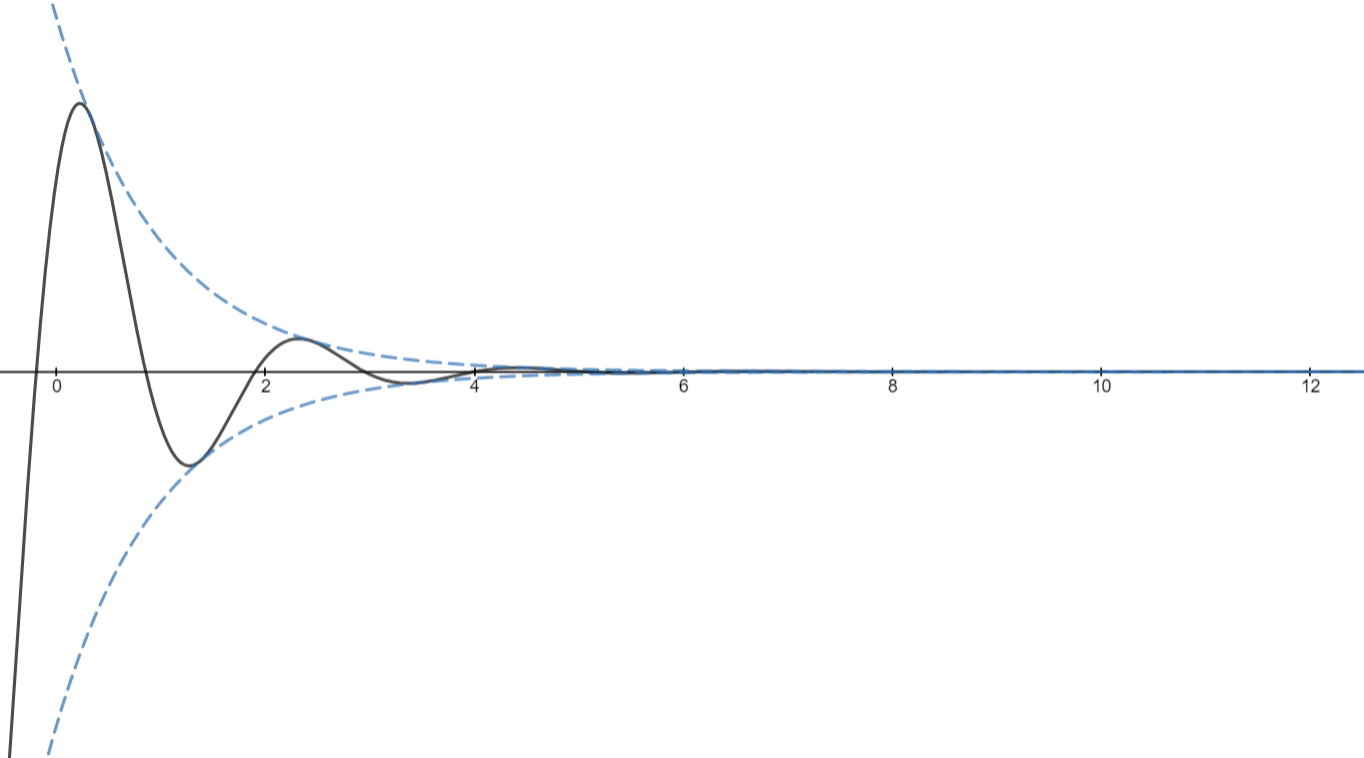
\includegraphics[width=0.5\textwidth]{./higherOrder/freeVibrs/underdamped.png}
\end{center}
Here, the exponential term dominates the limit, so
\begin{equation*}
	\lim\limits_{t \to 0}{Ae^{\frac{-b}{2m}t}\cos{(\omega t - \phi)}} = 0
\end{equation*}
meaning the mass's oscillation decays over time, bounded by the exponential curves. 

\ifodd\includeHigherOrderExamples\begin{example}
	A 250g mass is attached to a spring with a constant of $k = 10\text{N/m}$. The mechanical impedance is 3$\text{kg}{s}$. Initially, the mass is at $y(0)=-1\text{m}$ and $y'(0)=2\text{m/s}$. Find an expression for $y(t)$, the position of the mass at time $t$. Write any oscillations as a $\cos$ and a phase shift. Is the system underdamped, critically damped, or overdamped?
\end{example}
The IVP describing this scenario is
\begin{equation*}
	\begin{cases}
		\frac{1}{4}y'' + 3y' + 10y = 0 \\
		y(0) = -1 \\
		y'(0) = 2
	\end{cases}
\end{equation*}
Solving the auxiliary equation,
\begin{equation*}
	\frac{1}{4}r^2 + 3r + 10 = 0 \implies r = \frac{-3 \pm \sqrt{3^2 - 4(1/4)(10)}}{2(1/4)} = -6 \pm 2i
\end{equation*}
So, the general solution is
\begin{equation*}
	y = e^{-6t}\left(C_1\cos{(2t)} + C_2\sin{(2t)}\right)
\end{equation*}
Solving for $C_1$ and $C_2$,
\begin{equation*}
	y(0) = -1 = C_1 \implies C_1 = -1
\end{equation*}
\begin{equation*}
	y' = e^{-6t}\left(-2C_1\sin{(2t)} + 2C_2\cos{(2t)}\right) + \left(C_1\cos{(2t)} + C_2\sin{(2t)}\right) \cdot -6e^{-6t}
\end{equation*}
\begin{equation*}
	y'(0) = 2 = -6C_1 + 2C_2 \implies 2C_2 = -4 \implies C_2 = -2
\end{equation*}
Solving for $\phi$, keeping in mind that $C_1 < 0$,
\begin{equation*}
	\phi = \arctan{\frac{C_2}{C_2}} + \pi = \arctan{2} + \pi
\end{equation*}
So, our answer is (in units of meters)
\begin{equation*}
	y = \sqrt{(-1)^2 + (-2)^2}e^{-6t}\cos{\left(2t - \arctan{2} - \pi\right)} \approx 2.24e^{-6t}\cos{\left(2t - 4.25\right)}
\end{equation*}
Since our roots were complex, $\Delta < 0$. So, the system is underdamped.\fi